\documentclass[a4paper,11pt]{report}
\usepackage{amsmath}
\usepackage{amssymb}
\usepackage{graphicx}
\usepackage{wrapfig}
\usepackage{caption}
\usepackage{enumitem}
\usepackage{pdfpages}
\usepackage{multicol}
\usepackage[a4paper, left=3cm, right=3cm, top=3cm, bottom=3cm]{geometry}
\usepackage[ngerman]{babel}
\usepackage{hyperref}
\usepackage[x11names]{xcolor}
\usepackage{fancyhdr}
\pagestyle{fancy}
\usepackage{tikz}
\usetikzlibrary{calc}
\usepackage{titling}
\usepackage{fontspec}
\usepackage{titlesec}
\usepackage{moresize}
\usepackage{pgfplots}
\pgfplotsset{compat=1.15}

\usepackage{mathrsfs}
\usetikzlibrary{arrows}

% font setup
\newfontfamily{\newUpperTitleFont}{Bebas Neue}
\newfontfamily{\newLowerTitleFont}{Tex Gyre Heros Bold}

% font init
\titleformat{\part}[display]{\centering\HUGE\scshape\newUpperTitleFont\color{SlateBlue4}}{\partname~\thepart}{10pt}{}
\titleformat{\chapter}{\Huge\bfseries\newUpperTitleFont\color{SlateBlue4}}{\thechapter}{1em}{}
\titleformat*{\section}{\Large\bfseries\newLowerTitleFont\color{SlateBlue3}}
\titleformat*{\subsection}{\large\bfseries\newLowerTitleFont\color{SlateBlue2}}

% hyperlink setup
\hypersetup{
    colorlinks,
    citecolor=black,
    filecolor=black,
    linkcolor=SlateBlue3,
    urlcolor=black
}

% clear Footer
\fancyfoot{}

% Header
\fancyhead[L]{Niklas Fister}
\fancyhead[C]{Kantonnschule - Mathematik}
\fancyhead[R]{\thepage}
\renewcommand{\headrulewidth}{1pt}

\fancypagestyle{plain}{
    \fancyhead[L]{Niklas Fister}
    \fancyhead[C]{Kantonnschule - Mathematik}
    \fancyhead[R]{\thepage}
    \renewcommand{\headrulewidth}{1pt}
}

% Title
\title{\Huge\textbf{Bericht Physik - Lautsprecher}}
\author{Niklas Fister}
\date{\today}

% makeing title
\begin{document}
\pagenumbering{Roman}

% pretitle
%
\includepdf[scale=1.05]{resources/pdf/Title.pdf}

% own title
\begin{titlepage}
    \centering
    \begin{tikzpicture}[remember picture, overlay]
        \draw[line width=5pt, line cap=round, color=SlateBlue1, rounded corners=5pt]($(current page.west)+(1cm, 0)$) -- ($(current page.north west)+(1cm, -1cm)$) -- ($(current page.north)+(0, -1cm)$);
        \draw[line width=5pt, line cap=round, color=SlateBlue1, rounded corners=5pt]($(current page.east)+(-1cm, 0)$) -- ($(current page.south east)+(-1cm, 1cm)$) -- ($(current page.south)+(0, 1cm)$);
    \end{tikzpicture}

    % background
    \tikz[remember picture,overlay] \node[opacity=0.3,inner sep=0pt] at (current page.center){
\includegraphics[width=\paperwidth - 4cm, height=\paperheight - 4cm]{resources/images/Mandelbrotmenge.jpg}};
    % Start Text
    \vspace{4cm}

    % the title
    {\newUpperTitleFont\thetitle\par}
    \vspace{1cm}

    % the autors
    {\theauthor\par}
    \vspace{.5cm}

    % date
    {\thedate\par}
    \vspace{5cm}

    % showcase
    %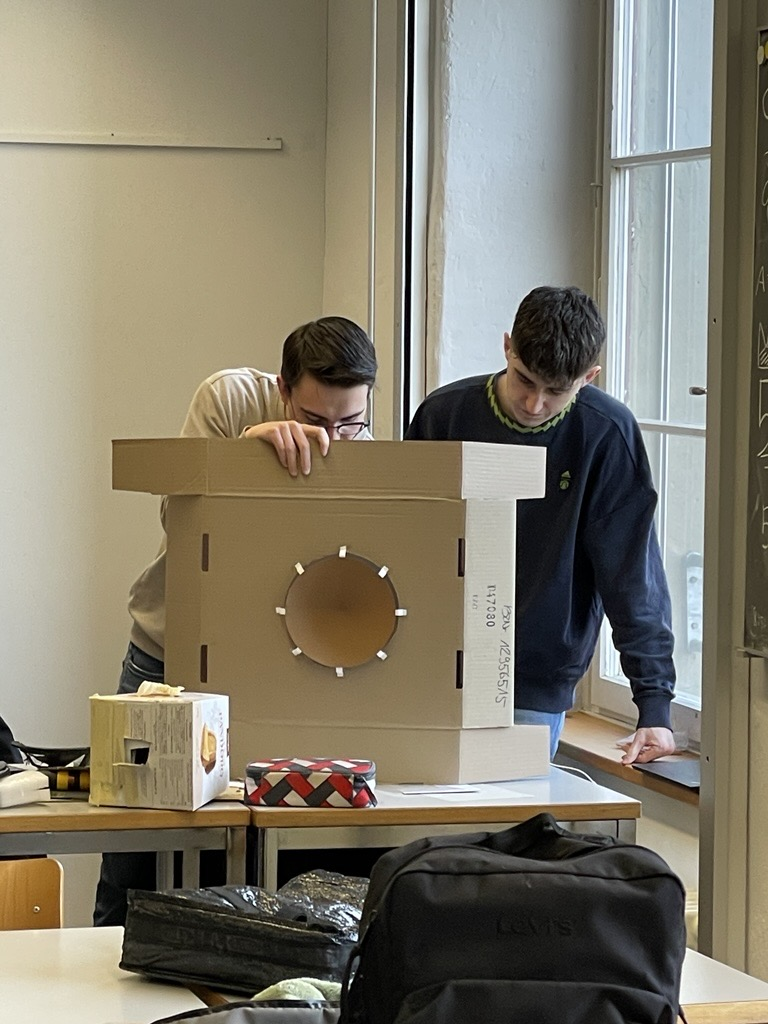
\includegraphics[width=.4\linewidth]{resources/images/Andrin_Cyrill_building.jpeg}
\end{titlepage}
\part{Analysis}
\chapter{Graphischer Zusammenhang der Analysis}
\section{Bedeutung der Ableitung}
Die Ableitung ist die Funktion, welche die Steigung einer anderen Funktion an einem bestimmten Wert für $x$ angibt. 

Es lässt sich somit an dem $y$-Wert der abgeleiteten Funktion die Steigung graphisch, sowie auch numerisch bestimmen.\\

Um dies algebraisch zu bestimmen verwendet man den Limes:
\begin{equation}
    f'(x) = \lim_{h \to 0} \frac{f(x+h) - f(x)}{h}
\end{equation}

Diese Formel ist nichts weiteres als das vorhin erwähnte $\frac{\Delta y}{\Delta x}$, jedoch wurde hier die Funktion eingesetzt.

Man nimmt einen Punkt $x$, sowieso den um $h$ vergrösserten und erhält damit die Formel. Durch den Limes wird der Abstand $h$ 0 angenähert und somit erhält man die Tangente.
\begin{center}
    \begin{tikzpicture}
        \begin{axis}[
            axis lines = middle,
            width=.8\linewidth,
            ymin=-25,ymax=20,
            xmin=-5,xmax=10,
            xlabel=$x$,
            ylabel=$y$,
        ]
        \addplot[smooth, thick, SlateBlue4, domain=-5:10]{x^3 - 3*x^2 - 9*x + 5}; 
        \addplot[smooth, thick, SlateBlue1, domain=-5:10]{3*x^2-6*x-9}; 
        \legend{$f(x) = x^3 - 3\cdot x^2 - 9\cdot x + 5$, $f'(x) = 3\cdot x^2 - 6\cdot x - 9$}
        \end{axis}
    \end{tikzpicture}
\end{center}

\noindent Dies lässt sich in dieser Grafik gut erkennen. Die abgeleitete Funktion $f'(x)$ gibt die Steigung der Funktion $f(x)$ an.

\newpage
\section{Graphische Darstellung des Differential}
\begin{minipage}{.5\textwidth}
    Um das Differential zu erhalten, versucht man die Funktion einer Tangente an der Stelle anzunähern. Um eine Annäherung zu erhlaten rechnet man $\frac{\Delta x}{\Delta y}$. Ziel ist es dabei das $\Delta x$ gegen 0 zu nähern. Wenn es unendlich klein wird, erhält man die tatsächliche Tangente.
\end{minipage}
\hspace{0.1\textwidth}
\begin{minipage}{.4\textwidth}
    \begin{tikzpicture}[line cap=round,line join=round,>=triangle 45]
        \begin{axis}[
        x=.5cm,y=.5cm,
        axis lines=middle,
        xmin=-5,
        xmax=5,
        ymin=-1,
        ymax=10,
        xtick={-4,-2,...,4},
        ytick={-1,0,5,10},]
        \clip(-5,-1) rectangle (5,10);
        % the functions
        \draw[line width=1pt,smooth,samples=100,domain=-5:5] plot(\x,{(\x)^(2)});
        \draw [line width=1pt,color=SlateBlue1,domain=-5:5] plot(\x,{(-1.2204223944078445--1.9330321397125094*\x)/0.7126097453046649});
        \draw [line width=1pt,color=OrangeRed1,domain=-5:5] plot(\x,{(-1--2*\x)/1});
        % the lines for illustration
        \draw [line width=1pt,color=SeaGreen3, dash pattern=on 1pt off 2pt] (1,1)-- (1.712609745304665,1);
        \draw [line width=1pt,color=SeaGreen3, dash pattern=on 1pt off 2pt] (1.712609745304665,1)-- (1.712609745304665,2.9330321397125094);
        % The two points
        \draw [color=SeaGreen3, fill=SeaGreen3] (1,1) circle (1.5pt);
        \draw [color=SeaGreen3 , fill=SeaGreen3] (1.712609745304665,2.9330321397125094) circle (1.5pt);
        \begin{scriptsize}
            \draw[color=SeaGreen3] (1.6,0.6) node {$\Delta x$};
            \draw[color=SeaGreen3] (2.3,1.8) node {$\Delta y$};
            \draw[color=SeaGreen3] (.5,1.2) node {$A$};
            \draw[color=SeaGreen3] (1.3,3.2) node {$B$};
            \draw[color=black] (1.5,9) node [scale=0.7] {$f(x) = x^2$};
            \draw[color=OrangeRed1] (3.5,4) node [scale=0.5] {$Tangente$};
            \draw[color=SlateBlue1] (2,8) node [scale=0.5] {$Approximation$};
        \end{scriptsize}
        \end{axis}
    \end{tikzpicture}
\end{minipage}

In einzelnen Etappen darstellt sieht das folgendermassen aus: \\

\vspace{.5cm}

\begin{minipage}{.5\textwidth}
    \begin{center}
        \begin{tikzpicture}[line cap=round,line join=round,>=triangle 45]
            \begin{axis}[
            x=.5cm,y=.5cm,
            axis lines=middle,
            xmin=-5,
            xmax=5,
            ymin=-1,
            ymax=10,
            xtick={-4,-2,...,4},
            ytick={-1,0,5,10},]
            \clip(-5,-1) rectangle (5,10);
            % the functions
            \draw[line width=1pt,smooth,samples=100,domain=-5:5] plot(\x,{(\x)^(2)});
            \draw [line width=1pt,color=SlateBlue1,domain=-5:5] plot(\x,{(-0.5866610252431241--1.0013527903985366*\x)/0.4146917651554125});
            \draw [line width=1pt,color=OrangeRed1,domain=-5:5] plot(\x,{(-1--2*\x)/1});
            \draw [color=SeaGreen3, fill=SeaGreen3] (1,1) circle (1.5pt);
            \begin{scriptsize}
                \draw[color=black] (1.5,9) node [scale=0.7] {$f(x) = x^2$};
                \draw[color=OrangeRed1] (3.5,4) node [scale=0.5] {$Tangente$};
                \draw[color=SlateBlue1] (2.2,8) node [scale=0.5] {$Approximation$};
            \end{scriptsize}
            \end{axis}
        \end{tikzpicture}
    \end{center}
\end{minipage}
\begin{minipage}{.5\textwidth}
    \begin{center}
        \begin{tikzpicture}[line cap=round,line join=round,>=triangle 45]
            \begin{axis}[
            x=.5cm,y=.5cm,
            axis lines=middle,
            xmin=-5,
            xmax=5,
            ymin=-1,
            ymax=10,
            xtick={-4,-2,...,4},
            ytick={-1,0,5,10},]
            \clip(-5,-1) rectangle (5,10);
            % the functions
            \draw[line width=1pt,smooth,samples=100,domain=-5:5] plot(\x,{(\x)^(2)});
            \draw [line width=1pt,color=SlateBlue1,domain=-5:5] plot(\x,{(-0.26685783030006305--0.4857860814489958*\x)/0.21892825114893277});
            \draw [line width=1pt,color=OrangeRed1,domain=-5:5] plot(\x,{(-1--2*\x)/1});
            \draw [color=SeaGreen3, fill=SeaGreen3] (1,1) circle (1.5pt);
            \begin{scriptsize}
                \draw[color=black] (1.5,9) node [scale=0.7] {$f(x) = x^2$};
                \draw[color=OrangeRed1] (3.5,4) node [scale=0.5] {$Tangente$};
                \draw[color=SlateBlue1] (2.4,8) node [scale=0.5] {$Approximation$};
            \end{scriptsize}
            \end{axis}
        \end{tikzpicture}
    \end{center}
\end{minipage}

\vspace{.5cm}

\begin{minipage}{.5\textwidth}
    \begin{center}
        \begin{tikzpicture}[line cap=round,line join=round,>=triangle 45]
            \begin{axis}[
            x=.5cm,y=.5cm,
            axis lines=middle,
            xmin=-5,
            xmax=5,
            ymin=-1,
            ymax=10,
            xtick={-4,-2,...,4},
            ytick={-1,0,5,10},]
            \clip(-5,-1) rectangle (5,10);
            % the functions
            \draw[line width=1pt,smooth,samples=100,domain=-5:5] plot(\x,{(\x)^(2)});
            \draw [line width=1pt,color=SlateBlue1,domain=-5:5] plot(\x,{(-0.13280363043648746--0.2515148962434772*\x)/0.11871126580698976});
            \draw [line width=1pt,color=OrangeRed1,domain=-5:5] plot(\x,{(-1--2*\x)/1});
            \draw [color=SeaGreen3, fill=SeaGreen3] (1,1) circle (1.5pt);
            \begin{scriptsize}
                \draw[color=black] (1.5,9) node [scale=0.7] {$f(x) = x^2$};
                \draw[color=OrangeRed1] (3.5,4) node [scale=0.5] {$Tangente$};
                \draw[color=SlateBlue1] (2.5,8) node [scale=0.5] {$Approximation$};
            \end{scriptsize}
            \end{axis}
        \end{tikzpicture}
    \end{center}
\end{minipage}
\begin{minipage}{.5\textwidth}
    \begin{center}
        \begin{tikzpicture}[line cap=round,line join=round,>=triangle 45]
            \begin{axis}[
            x=.5cm,y=.5cm,
            axis lines=middle,
            xmin=-5,
            xmax=5,
            ymin=-1,
            ymax=10,
            xtick={-4,-2,...,4},
            ytick={-1,0,5,10},]
            \clip(-5,-1) rectangle (5,10);
            % the functions
            \draw[line width=1pt,smooth,samples=100,domain=-5:5] plot(\x,{(\x)^(2)});
            \draw [line width=1pt,color=SlateBlue1,domain=-5:5] plot(\x,{(-0.025258746556910072--0.04990981780037007*\x)/0.02465107124346});
            \draw [line width=1pt,color=OrangeRed1,domain=-5:5] plot(\x,{(-1--2*\x)/1});
            \draw [color=SeaGreen3, fill=SeaGreen3] (1,1) circle (1.5pt);
            \begin{scriptsize}
                \draw[color=black] (1.5,9) node [scale=0.7] {$f(x) = x^2$};
                \draw[color=OrangeRed1] (3.5,4) node [scale=0.5] {$Tangente$};
                \draw[color=SlateBlue1] (2.6,8) node [scale=0.5] {$Approximation$};
            \end{scriptsize}
            \end{axis}
        \end{tikzpicture}
    \end{center}
\end{minipage}
Es ist klar eine tendenz zu sehen, dass sich die Geraden immer mehr annähern. Wenn durch den Limes nun dieser Abstand unendlich klein wird, konvergierren diese Geraden und werden zu einer.

\section{Graphische Darstellung des Integral}
\pgfplotsset{
    integral segments/.code={\pgfmathsetmacro\integralsegments{#1}},
    integral segments=1,
    integral/.style args={#1:#2}{
        ybar interval,
        domain=#1+((#2-#1)/\integralsegments)/2:#2+((#2-#1)/\integralsegments)/2,
        samples=\integralsegments+1,
        x filter/.code=\pgfmathparse{\pgfmathresult-((#2-#1)/\integralsegments)/2}
    },
    integralB segments/.code={\pgfmathsetmacro\integralsegmentsB{#1}},
    integralB segments=7,
    integralB/.style args={#1:#2}{
        ybar interval,
        domain=#1+((#2-#1)/\integralsegmentsB)/2:#2+((#2-#1)/\integralsegmentsB)/2,
        samples=\integralsegmentsB+1,
        x filter/.code=\pgfmathparse{\pgfmathresult-((#2-#1)/\integralsegmentsB)/2}
    },
    integralC segments/.code={\pgfmathsetmacro\integralsegmentsC{#1}},
    integralC segments=14,
    integralC/.style args={#1:#2}{
        ybar interval,
        domain=#1+((#2-#1)/\integralsegmentsC)/2:#2+((#2-#1)/\integralsegmentsC)/2,
        samples=\integralsegmentsC+1,
        x filter/.code=\pgfmathparse{\pgfmathresult-((#2-#1)/\integralsegmentsC)/2}
    },
    integralD segments/.code={\pgfmathsetmacro\integralsegmentsD{#1}},
    integralD segments=28,
    integralD/.style args={#1:#2}{
        ybar interval,
        domain=#1+((#2-#1)/\integralsegmentsD)/2:#2+((#2-#1)/\integralsegmentsD)/2,
        samples=\integralsegmentsD+1,
        x filter/.code=\pgfmathparse{\pgfmathresult-((#2-#1)/\integralsegmentsD)/2}
    },
    integralE segments/.code={\pgfmathsetmacro\integralsegmentsE{#1}},
    integralE segments=56,
    integralE/.style args={#1:#2}{
        ybar interval,
        domain=#1+((#2-#1)/\integralsegmentsE)/2:#2+((#2-#1)/\integralsegmentsE)/2,
        samples=\integralsegmentsE+1,
        x filter/.code=\pgfmathparse{\pgfmathresult-((#2-#1)/\integralsegmentsE)/2}
    },
}

\begin{minipage}{.5\textwidth}
    Die Herangehensweise um den Integral zu bestimmen ist folgender, dass man die Fläche unter der Funktion in Quadrate unterteilt, von welchen man die Fläche einfach berechnen kann.

    Da mit grossem $\Delta h$ die Fläche ungenau ist, nähert man dies 0 an, um sich der tatsächlichen Fläche unter der Kuzrve anzunähern.
\end{minipage}
\begin{minipage}{.5\textwidth}
    \begin{center}
        \begin{tikzpicture}[/pgf/declare function={f=(1/32)*x^2;}]
        \begin{axis}[
            width=0.9\linewidth,
            xmin=-1,
            xmax=20,
            ymin=-1,
            ymax=10,
            domain=0:20,
            samples=1000,
            axis lines=middle
        ]
        \addplot [thick] {f};
        \addplot [
            smooth,
            SlateBlue1,
            integral=14:16,
        ] {f};
        \begin{scriptsize}
            \draw[color=SeaGreen3] (17.5, 3.5) node [scale=0.8] {$f(x)$};
            \draw[color=SeaGreen3] (15, 7.5) node [scale=0.8] {$\Delta h$};
        \end{scriptsize}
        \legend{$f(x) = x^{-1}+1$}
        \end{axis}
        \end{tikzpicture}
    \end{center}
\end{minipage}

\vspace{.5cm}

\begin{minipage}{.5\textwidth}
    \begin{tikzpicture}[/pgf/declare function={f=(1/32)*x^2;}]
        \begin{axis}[
            width=0.9\linewidth,
            xmin=-1,
            xmax=20,
            ymin=-1,
            ymax=10,
            domain=0:20,
            samples=1000,
            axis lines=middle
        ]
        \addplot [thick] {f};
        \addplot [
            smooth,
            SlateBlue1,
            integralB=2:16,
        ] {f};
        \legend{$f(x) = x^{-1}+1$}
        \end{axis}
    \end{tikzpicture}
\end{minipage}
\begin{minipage}{.5\textwidth}
    \begin{tikzpicture}[/pgf/declare function={f=(1/32)*x^2;}]
        \begin{axis}[
            width=0.9\linewidth,
            xmin=-1,
            xmax=20,
            ymin=-1,
            ymax=10,
            domain=0:20,
            samples=1000,
            axis lines=middle
        ]
        \addplot [thick] {f};
        \addplot [
            smooth,
            SlateBlue1,
            integralC=2:16,
        ] {f};
        \legend{$f(x) = x^{-1}+1$}
        \end{axis}
    \end{tikzpicture}
\end{minipage}

\vspace{.5cm}

\begin{minipage}{.5\textwidth}
    \begin{tikzpicture}[/pgf/declare function={f=(1/32)*x^2;}]
        \begin{axis}[
            width=0.9\linewidth,
            xmin=-1,
            xmax=20,
            ymin=-1,
            ymax=10,
            domain=0:20,
            samples=1000,
            axis lines=middle
        ]
        \addplot [thick] {f};
        \addplot [
            smooth,
            SlateBlue1,
            integralD=2:16,
        ] {f};
        \legend{$f(x) = x^{-1}+1$}
        \end{axis}
    \end{tikzpicture}
\end{minipage}
\begin{minipage}{.5\textwidth}
    \begin{tikzpicture}[/pgf/declare function={f=(1/32)*x^2;}]
        \begin{axis}[
            width=0.9\linewidth,
            xmin=-1,
            xmax=20,
            ymin=-1,
            ymax=10,
            domain=0:20,
            samples=1000,
            axis lines=middle
        ]
        \addplot [thick] {f};
        \addplot [
            smooth,
            SlateBlue1,
            integralE=2:16,
        ] {f};
        \legend{$f(x) = x^{-1}+1$}
        \end{axis}
    \end{tikzpicture}
\end{minipage}

\vspace{.5cm}

\noindent Bei dem letzen Beispiel sieht man schon eine klare Annäherung an die tatsächliche Fläche, welche durch das Integral zu berechnen gilt.

\newpage
\section{Graphischer Zusammenhang der Beiden}
\begin{center}
    \begin{tikzpicture}
        \begin{axis}[
            axis lines = middle,
            width=.8\linewidth,
            ymin=-25,ymax=20,
            xmin=-4,xmax=4,
            xlabel=$x$,
            ylabel=$y$,
        ]
        % normal function
        \addplot[smooth, thick, black, domain=-4:4]{4*x^4-5*x^3};
        % derivative
        \addplot[smooth, thick, SlateBlue1, domain=-4:4]{16*x^3-15*x^2};
        % main integral
        \addplot[smooth, thick, SeaGreen3, domain=-4:4]{(4/5)*x^4-(5/4)*x^3}; 
        % segments 
        \addplot[smooth, very thin, dash pattern=on 3pt off 5pt, SeaGreen3, domain=-2.5:3]{((4/5)*x^4-(5/4)*x^3) + 1};
        \addplot[smooth, very thin, dash pattern=on 3pt off 5pt, SeaGreen3, domain=-2.5:3]{((4/5)*x^4-(5/4)*x^3) + 2}; 
        \addplot[smooth, very thin, dash pattern=on 3pt off 5pt, SeaGreen3, domain=-2.5:3]{((4/5)*x^4-(5/4)*x^3) + 3}; 
        \addplot[smooth, very thin, dash pattern=on 3pt off 5pt, SeaGreen3, domain=-2.5:3]{((4/5)*x^4-(5/4)*x^3) + 4}; 
        \addplot[smooth, very thin, dash pattern=on 3pt off 5pt, SeaGreen3, domain=-2.5:3]{((4/5)*x^4-(5/4)*x^3) + 5}; 
        \addplot[smooth, very thin, dash pattern=on 3pt off 5pt, SeaGreen3, domain=-2.5:3]{((4/5)*x^4-(5/4)*x^3) + 6};
        \addplot[smooth, very thin, dash pattern=on 3pt off 5pt, SeaGreen3, domain=-2.5:3]{((4/5)*x^4-(5/4)*x^3) + 7}; 
        \addplot[smooth, very thin, dash pattern=on 3pt off 5pt, SeaGreen3, domain=-2.5:3]{((4/5)*x^4-(5/4)*x^3) + 8}; 
        \addplot[smooth, very thin, dash pattern=on 3pt off 5pt, SeaGreen3, domain=-2.5:3]{((4/5)*x^4-(5/4)*x^3) + 9}; 
        \addplot[smooth, very thin, dash pattern=on 3pt off 5pt, SeaGreen3, domain=-2.5:3]{((4/5)*x^4-(5/4)*x^3) + 10};
        \addplot[smooth, very thin, dash pattern=on 3pt off 5pt, SeaGreen3, domain=-2.5:3]{((4/5)*x^4-(5/4)*x^3) + 11};
        \addplot[smooth, very thin, dash pattern=on 3pt off 5pt, SeaGreen3, domain=-2.5:3]{((4/5)*x^4-(5/4)*x^3) + 12};
        \addplot[smooth, very thin, dash pattern=on 3pt off 5pt, SeaGreen3, domain=-2.5:3]{((4/5)*x^4-(5/4)*x^3) + 13};
        \addplot[smooth, very thin, dash pattern=on 3pt off 5pt, SeaGreen3, domain=-2.5:3]{((4/5)*x^4-(5/4)*x^3) + 14};
        \addplot[smooth, very thin, dash pattern=on 3pt off 5pt, SeaGreen3, domain=-2.5:3]{((4/5)*x^4-(5/4)*x^3) + 15};
        \addplot[smooth, very thin, dash pattern=on 3pt off 5pt, SeaGreen3, domain=-2.5:3]{((4/5)*x^4-(5/4)*x^3) + 16};
        \addplot[smooth, very thin, dash pattern=on 3pt off 5pt, SeaGreen3, domain=-2.5:3]{((4/5)*x^4-(5/4)*x^3) + 17};
        \addplot[smooth, very thin, dash pattern=on 3pt off 5pt, SeaGreen3, domain=-2.5:3]{((4/5)*x^4-(5/4)*x^3) + 18};
        \addplot[smooth, very thin, dash pattern=on 3pt off 5pt, SeaGreen3, domain=-2.5:3]{((4/5)*x^4-(5/4)*x^3) + 19};
        \addplot[smooth, very thin, dash pattern=on 3pt off 5pt, SeaGreen3, domain=-2.5:3]{((4/5)*x^4-(5/4)*x^3) + 20};
        \addplot[smooth, very thin, dash pattern=on 3pt off 5pt, SeaGreen3, domain=-2.5:3]{((4/5)*x^4-(5/4)*x^3) - 1};
        \addplot[smooth, very thin, dash pattern=on 3pt off 5pt, SeaGreen3, domain=-2.5:3]{((4/5)*x^4-(5/4)*x^3) - 2}; 
        \addplot[smooth, very thin, dash pattern=on 3pt off 5pt, SeaGreen3, domain=-2.5:3]{((4/5)*x^4-(5/4)*x^3) - 3}; 
        \addplot[smooth, very thin, dash pattern=on 3pt off 5pt, SeaGreen3, domain=-2.5:3]{((4/5)*x^4-(5/4)*x^3) - 4}; 
        \addplot[smooth, very thin, dash pattern=on 3pt off 5pt, SeaGreen3, domain=-2.5:3]{((4/5)*x^4-(5/4)*x^3) - 5}; 
        \addplot[smooth, very thin, dash pattern=on 3pt off 5pt, SeaGreen3, domain=-2.5:3]{((4/5)*x^4-(5/4)*x^3) - 6};
        \addplot[smooth, very thin, dash pattern=on 3pt off 5pt, SeaGreen3, domain=-2.5:3]{((4/5)*x^4-(5/4)*x^3) - 7}; 
        \addplot[smooth, very thin, dash pattern=on 3pt off 5pt, SeaGreen3, domain=-2.5:3]{((4/5)*x^4-(5/4)*x^3) - 8}; 
        \addplot[smooth, very thin, dash pattern=on 3pt off 5pt, SeaGreen3, domain=-2.5:3]{((4/5)*x^4-(5/4)*x^3) - 9}; 
        \addplot[smooth, very thin, dash pattern=on 3pt off 5pt, SeaGreen3, domain=-2.5:3]{((4/5)*x^4-(5/4)*x^3) - 10};
        \addplot[smooth, very thin, dash pattern=on 3pt off 5pt, SeaGreen3, domain=-2.5:3]{((4/5)*x^4-(5/4)*x^3) - 11};
        \addplot[smooth, very thin, dash pattern=on 3pt off 5pt, SeaGreen3, domain=-2.5:3]{((4/5)*x^4-(5/4)*x^3) - 12};
        \addplot[smooth, very thin, dash pattern=on 3pt off 5pt, SeaGreen3, domain=-2.5:3]{((4/5)*x^4-(5/4)*x^3) - 13};
        \addplot[smooth, very thin, dash pattern=on 3pt off 5pt, SeaGreen3, domain=-2.5:3]{((4/5)*x^4-(5/4)*x^3) - 14};
        \addplot[smooth, very thin, dash pattern=on 3pt off 5pt, SeaGreen3, domain=-2.5:3]{((4/5)*x^4-(5/4)*x^3) - 15};
        \addplot[smooth, very thin, dash pattern=on 3pt off 5pt, SeaGreen3, domain=-2.5:3]{((4/5)*x^4-(5/4)*x^3) - 16};
        \addplot[smooth, very thin, dash pattern=on 3pt off 5pt, SeaGreen3, domain=-2.5:3]{((4/5)*x^4-(5/4)*x^3) - 17};
        \addplot[smooth, very thin, dash pattern=on 3pt off 5pt, SeaGreen3, domain=-2.5:3]{((4/5)*x^4-(5/4)*x^3) - 18};
        \addplot[smooth, very thin, dash pattern=on 3pt off 5pt, SeaGreen3, domain=-2.5:3]{((4/5)*x^4-(5/4)*x^3) - 19};
        \addplot[smooth, very thin, dash pattern=on 3pt off 5pt, SeaGreen3, domain=-2.5:3]{((4/5)*x^4-(5/4)*x^3) - 20};
        \addplot[smooth, very thin, dash pattern=on 3pt off 5pt, SeaGreen3, domain=-2.5:3]{((4/5)*x^4-(5/4)*x^3) - 21};
        \addplot[smooth, very thin, dash pattern=on 3pt off 5pt, SeaGreen3, domain=-2.5:3]{((4/5)*x^4-(5/4)*x^3) - 22};
        \addplot[smooth, very thin, dash pattern=on 3pt off 5pt, SeaGreen3, domain=-2.5:3]{((4/5)*x^4-(5/4)*x^3) - 23};
        \addplot[smooth, very thin, dash pattern=on 3pt off 5pt, SeaGreen3, domain=-2.5:3]{((4/5)*x^4-(5/4)*x^3) - 24};
        \addplot[smooth, very thin, dash pattern=on 3pt off 5pt, SeaGreen3, domain=-2.5:3]{((4/5)*x^4-(5/4)*x^3) - 25};
        \addplot[smooth, very thin, dash pattern=on 3pt off 5pt, SeaGreen3, domain=-2.5:3]{((4/5)*x^4-(5/4)*x^3) - 26};
        \addplot[smooth, very thin, dash pattern=on 3pt off 5pt, SeaGreen3, domain=-2.5:3]{((4/5)*x^4-(5/4)*x^3) - 27};
        \addplot[smooth, very thin, dash pattern=on 3pt off 5pt, SeaGreen3, domain=-2.5:3]{((4/5)*x^4-(5/4)*x^3) - 28};
        \addplot[smooth, very thin, dash pattern=on 3pt off 5pt, SeaGreen3, domain=-2.5:3]{((4/5)*x^4-(5/4)*x^3) - 29};
        \addplot[smooth, very thin, dash pattern=on 3pt off 5pt, SeaGreen3, domain=-2.5:3]{((4/5)*x^4-(5/4)*x^3) - 30};
        \addplot[smooth, very thin, dash pattern=on 3pt off 5pt, SeaGreen3, domain=-2.5:3]{((4/5)*x^4-(5/4)*x^3) - 31};
        \addplot[smooth, very thin, dash pattern=on 3pt off 5pt, SeaGreen3, domain=-2.5:3]{((4/5)*x^4-(5/4)*x^3) - 32};
        \addplot[smooth, very thin, dash pattern=on 3pt off 5pt, SeaGreen3, domain=-2.5:3]{((4/5)*x^4-(5/4)*x^3) - 33};
        \addplot[smooth, very thin, dash pattern=on 3pt off 5pt, SeaGreen3, domain=-2.5:3]{((4/5)*x^4-(5/4)*x^3) - 34};
        \addplot[smooth, very thin, dash pattern=on 3pt off 5pt, SeaGreen3, domain=-2.5:3]{((4/5)*x^4-(5/4)*x^3) - 35};
        \addplot[smooth, very thin, dash pattern=on 3pt off 5pt, SeaGreen3, domain=-2.5:3]{((4/5)*x^4-(5/4)*x^3) - 36};
        \addplot[smooth, very thin, dash pattern=on 3pt off 5pt, SeaGreen3, domain=-2.5:3]{((4/5)*x^4-(5/4)*x^3) - 37};
        \addplot[smooth, very thin, dash pattern=on 3pt off 5pt, SeaGreen3, domain=-2.5:3]{((4/5)*x^4-(5/4)*x^3) - 38};
        \addplot[smooth, very thin, dash pattern=on 3pt off 5pt, SeaGreen3, domain=-2.5:3]{((4/5)*x^4-(5/4)*x^3) - 39};
        \addplot[smooth, very thin, dash pattern=on 3pt off 5pt, SeaGreen3, domain=-2.5:3]{((4/5)*x^4-(5/4)*x^3) - 40};
        \addplot[smooth, very thin, dash pattern=on 3pt off 5pt, SeaGreen3, domain=-2.5:3]{((4/5)*x^4-(5/4)*x^3) - 41};
        \addplot[smooth, very thin, dash pattern=on 3pt off 5pt, SeaGreen3, domain=-2.5:3]{((4/5)*x^4-(5/4)*x^3) - 42};
        \addplot[smooth, very thin, dash pattern=on 3pt off 5pt, SeaGreen3, domain=-2.5:3]{((4/5)*x^4-(5/4)*x^3) - 43};
        \addplot[smooth, very thin, dash pattern=on 3pt off 5pt, SeaGreen3, domain=-2.5:3]{((4/5)*x^4-(5/4)*x^3) - 44};
        \addplot[smooth, very thin, dash pattern=on 3pt off 5pt, SeaGreen3, domain=-2.5:3]{((4/5)*x^4-(5/4)*x^3) - 45};
        \addplot[smooth, very thin, dash pattern=on 3pt off 5pt, SeaGreen3, domain=-2.5:3]{((4/5)*x^4-(5/4)*x^3) - 46};
        \addplot[smooth, very thin, dash pattern=on 3pt off 5pt, SeaGreen3, domain=-2.5:3]{((4/5)*x^4-(5/4)*x^3) - 47};
        \addplot[smooth, very thin, dash pattern=on 3pt off 5pt, SeaGreen3, domain=-2.5:3]{((4/5)*x^4-(5/4)*x^3) - 48};
        \addplot[smooth, very thin, dash pattern=on 3pt off 5pt, SeaGreen3, domain=-2.5:3]{((4/5)*x^4-(5/4)*x^3) - 49};
        \addplot[smooth, very thin, dash pattern=on 3pt off 5pt, SeaGreen3, domain=-2.5:3]{((4/5)*x^4-(5/4)*x^3) - 50};
        \addplot[smooth, very thin, dash pattern=on 3pt off 5pt, SeaGreen3, domain=-2.5:3]{((4/5)*x^4-(5/4)*x^3) - 51};
        \addplot[smooth, very thin, dash pattern=on 3pt off 5pt, SeaGreen3, domain=-2.5:3]{((4/5)*x^4-(5/4)*x^3) - 52};
        \addplot[smooth, very thin, dash pattern=on 3pt off 5pt, SeaGreen3, domain=-2.5:3]{((4/5)*x^4-(5/4)*x^3) - 53};
        \addplot[smooth, very thin, dash pattern=on 3pt off 5pt, SeaGreen3, domain=-2.5:3]{((4/5)*x^4-(5/4)*x^3) - 54};
        \addplot[smooth, very thin, dash pattern=on 3pt off 5pt, SeaGreen3, domain=-2.5:3]{((4/5)*x^4-(5/4)*x^3) - 55};
        \addplot[smooth, very thin, dash pattern=on 3pt off 5pt, SeaGreen3, domain=-2.5:3]{((4/5)*x^4-(5/4)*x^3) - 56};
        \addplot[smooth, very thin, dash pattern=on 3pt off 5pt, SeaGreen3, domain=-2.5:3]{((4/5)*x^4-(5/4)*x^3) - 57};
        \addplot[smooth, very thin, dash pattern=on 3pt off 5pt, SeaGreen3, domain=-2.5:3]{((4/5)*x^4-(5/4)*x^3) - 58};
        \addplot[smooth, very thin, dash pattern=on 3pt off 5pt, SeaGreen3, domain=-2.5:3]{((4/5)*x^4-(5/4)*x^3) - 59};
        \addplot[smooth, very thin, dash pattern=on 3pt off 5pt, SeaGreen3, domain=-2.5:3]{((4/5)*x^4-(5/4)*x^3) - 60};
        \addplot[smooth, very thin, dash pattern=on 3pt off 5pt, SeaGreen3, domain=-2.5:3]{((4/5)*x^4-(5/4)*x^3) - 61};
        \addplot[smooth, very thin, dash pattern=on 3pt off 5pt, SeaGreen3, domain=-2.5:3]{((4/5)*x^4-(5/4)*x^3) - 62};
        \addplot[smooth, very thin, dash pattern=on 3pt off 5pt, SeaGreen3, domain=-2.5:3]{((4/5)*x^4-(5/4)*x^3) - 63};
        \addplot[smooth, very thin, dash pattern=on 3pt off 5pt, SeaGreen3, domain=-2.5:3]{((4/5)*x^4-(5/4)*x^3) - 64};
        \addplot[smooth, very thin, dash pattern=on 3pt off 5pt, SeaGreen3, domain=-2.5:3]{((4/5)*x^4-(5/4)*x^3) - 65};
        \addplot[smooth, very thin, dash pattern=on 3pt off 5pt, SeaGreen3, domain=-2.5:3]{((4/5)*x^4-(5/4)*x^3) - 66};
        \addplot[smooth, very thin, dash pattern=on 3pt off 5pt, SeaGreen3, domain=-2.5:3]{((4/5)*x^4-(5/4)*x^3) - 67};
        \addplot[smooth, very thin, dash pattern=on 3pt off 5pt, SeaGreen3, domain=-2.5:3]{((4/5)*x^4-(5/4)*x^3) - 68};
        \addplot[smooth, very thin, dash pattern=on 3pt off 5pt, SeaGreen3, domain=-2.5:3]{((4/5)*x^4-(5/4)*x^3) - 69};
        \addplot[smooth, very thin, dash pattern=on 3pt off 5pt, SeaGreen3, domain=-2.5:3]{((4/5)*x^4-(5/4)*x^3) - 70};
        \addplot[smooth, very thin, dash pattern=on 3pt off 5pt, SeaGreen3, domain=-2.5:3]{((4/5)*x^4-(5/4)*x^3) - 71};
        \addplot[smooth, very thin, dash pattern=on 3pt off 5pt, SeaGreen3, domain=-2.5:3]{((4/5)*x^4-(5/4)*x^3) - 72};
        \addplot[smooth, very thin, dash pattern=on 3pt off 5pt, SeaGreen3, domain=-2.5:3]{((4/5)*x^4-(5/4)*x^3) - 73};
        \addplot[smooth, very thin, dash pattern=on 3pt off 5pt, SeaGreen3, domain=-2.5:3]{((4/5)*x^4-(5/4)*x^3) - 74};
        \addplot[smooth, very thin, dash pattern=on 3pt off 5pt, SeaGreen3, domain=-2.5:3]{((4/5)*x^4-(5/4)*x^3) - 75};
        \legend{$f(x)$, $f'(x)$, $F(x)$}
        \end{axis}
    \end{tikzpicture}
\end{center}
Anhand dieses Graphen lässt sich der Graphische Zusammenhang der Funktion, ihrer Ableitung und ihrer Stammfunktion gut erklären.

Die Funktion $f'(x)$ hat an jeder Stelle $x$ den Wert der Steigung der Funktion $x$. Anfangs hat $f(x)$ eine negative Steigung und somit sind die Werte der Ableitung ebenfalls negative. Sobald die Funktion jedoch wieder eine positive Steigung hat, sind auch die Werte der Ableitung im positiven. Dies ist immer so zu erkennen.

Die Stammfunktion $F(x)$ gibt die Fläche unter dem Graphen an und ist die Gegenfunktion der Ableitung. Der Wert der Funktion $f(x)$ gibt zu jedem Punkt die Steigung der Stammfunktion vor.
Da diese Steigung überall für eine Punkt $x$ auf der $y-Achse$ identisch ist, muss man ein $+C$ addieren. Daraus resultieren die gestrichelten Graphen und man erhällt ein Richtungsfeld.
Zwischen den gestrichelten Linien gibt es noch viele weitere Funktionen, denn man kann den Wert für $C$ beliebig wählen $\rightarrow$ $C \in \mathbb{R}$ .

% Excercises
\newpage
\section{Übungen}
\begin{enumerate}
    \item \textbf{Erkläre in eigenen Worten, was die Ablteiung und die Stammfunktion einer Funktion ist und was sie geometrisch bedeutet.}
    \item \textbf{Berechne die Ableitung der folgenden Funktionen:}
    \begin{multicols}{2}
        \begin{enumerate}[label=(\alph*)]
            \item $f(x) = 3x^2 + 5x - 12$
            \item $f(x) = \sin(4x^2) + 3x^3$
            \item $f(x) = \frac{1}{x^2}$
            \item $f(x) = \sqrt{\frac{5}{x^2}}$
            \item $f(x) = e^{3x}$
            \item $f(x) = \ln(2x)$
        \end{enumerate}
    \end{multicols}
    \item \textbf{Welche Funktionsgraphen sind Differentialgleichungen voneinander?}
    \begin{multicols}{3}
        \begin{center}
            \begin{tikzpicture}
                \begin{axis}[
                    axis lines=middle,
                    width=1.2\linewidth,
                    xmin=-3, xmax=3,
                    ymin=-10, ymax=10,
                    xlabel=$x$,
                    ylabel=$y$,
                ]
                \addplot[smooth, thick, SlateBlue2, domain=-3:3]{x^3 - 4*x};
                \end{axis}
            \end{tikzpicture}
        \end{center}
        \begin{center}
            \begin{tikzpicture}
                \begin{axis}[
                    axis lines=middle,
                    width=1.2\linewidth,
                    xmin=-3, xmax=5,
                    ymin=-5, ymax=5,
                    xlabel=$x$,
                    ylabel=$y$,
                    samples = 1000,
                ]
                \addplot[smooth, thick, SlateBlue2, domain=0:5]{ln(x)};
                \end{axis}
            \end{tikzpicture}
        \end{center}
        \begin{center}
            \begin{tikzpicture}
                \begin{axis}[
                    axis lines=middle,
                    width=1.2\linewidth,
                    xmin=-3, xmax=3,
                    ymin=-15, ymax=15,
                    xlabel=$x$,
                    ylabel=$y$,
                    trig format plots=rad,
                ]
                \addplot[smooth, thick, SlateBlue2, domain=-3:3]{12*cos(3*x)};
                \end{axis}
            \end{tikzpicture}
        \end{center}
        \begin{center}
            \begin{tikzpicture}
                \begin{axis}[
                    axis lines=middle,
                    width=1.2\linewidth,
                    xmin=-5, xmax=5,
                    ymin=-10, ymax=10,
                    xlabel=$x$,
                    ylabel=$y$,
                ]
                \addplot[smooth, thick, SlateBlue2, domain=-5:5]{(1/4)*x^4 - 2*x^2};
                \end{axis}
            \end{tikzpicture}
        \end{center}
        \begin{center}
            \begin{tikzpicture}
                \begin{axis}[
                    axis lines=middle,
                    width=1.2\linewidth,
                    xmin=-3, xmax=3,
                    ymin=-6, ymax=6,
                    xlabel=$x$,
                    ylabel=$y$,
                    trig format plots=rad,
                ]
                \addplot[smooth, thick, SlateBlue2, domain=-3:3]{4*sin(3*x)};
                \end{axis}
            \end{tikzpicture}
        \end{center}
        \begin{center}
            \begin{tikzpicture}
                \begin{axis}[
                    axis lines=middle,
                    width=1.2\linewidth,
                    xmin=-3, xmax=3,
                    ymin=-5, ymax=5,
                    xlabel=$x$,
                    ylabel=$y$,
                ]
                \addplot[smooth, thick, SlateBlue2, domain=-3:0]{1/x};
                \addplot[smooth, thick, SlateBlue2, domain=0:3]{1/x};
                \end{axis}
            \end{tikzpicture}
        \end{center}
    \end{multicols}
\end{enumerate}
\end{document}